\pdfminorversion=7
\documentclass[aspectratio=169,xcolor={dvipsnames,table}]{beamer}

\usepackage[utf8]{inputenc}
\usepackage[T1]{fontenc}
\usepackage[spanish,es-nodecimaldot]{babel}
\usepackage{lmodern,amsmath,amssymb,cancel,booktabs,array,graphicx,ragged2e,tikz,pgfplots}
\usepackage{tcolorbox}
\pgfplotsset{compat=1.18}
\usetikzlibrary{arrows.meta,positioning,calc,fit,backgrounds,shapes.geometric,decorations.pathreplacing,patterns,babel}
\tcbuselibrary{skins}

\mode<presentation>{
  \usetheme{default}
  \usefonttheme{professionalfonts}
  \setbeamertemplate{navigation symbols}{}
  \setbeamertemplate{blocks}[rounded][shadow=false]
}

\setbeamersize{text margin left=0.45cm, text margin right=0.45cm}

% Paleta visual vibrante estilo estudio de ingenieria
\definecolor{visNavy}{HTML}{0B1E33}
\definecolor{visNavyMid}{HTML}{143658}
\definecolor{visBlue}{HTML}{1565C0}
\definecolor{visCyan}{HTML}{00ACC1}
\definecolor{visFluid}{HTML}{1E88E5}
\definecolor{visFluidLight}{HTML}{81D4FA}
\definecolor{visTeal}{HTML}{00897B}
\definecolor{visGreen}{HTML}{2E7D32}
\definecolor{visAmber}{HTML}{F59E0B}
\definecolor{visOrange}{HTML}{E65100}
\definecolor{visRed}{HTML}{C62828}
\definecolor{visPink}{HTML}{D81B60}
\definecolor{visPaper}{HTML}{F4F7FA}
\definecolor{visInk}{HTML}{162433}
\definecolor{visMuted}{HTML}{5C6F84}
\definecolor{visSteel}{HTML}{90A4AE}
\definecolor{visSteelDark}{HTML}{455A64}

\setbeamercolor{background canvas}{bg=visPaper}
\setbeamercolor{normal text}{fg=visInk,bg=visPaper}
\setbeamerfont{frametitle}{size=\fontsize{12.5}{15}\selectfont,series=\bfseries}

\newcommand{\visualLogo}[1]{%
  \IfFileExists{img/#1}{\includegraphics[height=0.52cm]{img/#1}}{\textbf{\color{white}IIIEPE}}%
}

% Header visual limpio para diapositivas de contenido
\newcommand{\visHeader}[2]{%
  \begin{tikzpicture}[remember picture,overlay]
    \fill[visNavy] (current page.north west) rectangle ([yshift=-1.05cm]current page.north east);
    \fill[visAmber] ([yshift=-1.05cm]current page.north west) rectangle ([yshift=-1.12cm]current page.north east);
    \node[anchor=west,text=white,font=\fontsize{12.5}{15}\selectfont\bfseries]
      at ([xshift=0.48cm,yshift=-0.42cm]current page.north west) {#1};
    \node[anchor=west,text=visFluidLight,font=\fontsize{7.5}{9}\selectfont]
      at ([xshift=0.48cm,yshift=-0.82cm]current page.north west) {#2};
    \node[anchor=east]
      at ([xshift=-0.42cm,yshift=-0.52cm]current page.north west -| current page.north east) {\visualLogo{logo-iiiepe-blanco.png}};
  \end{tikzpicture}%
  \vspace*{0.92cm}%
}

% Footer discreto para contenido
\setbeamertemplate{footline}{%
  \leavevmode\hbox{%
    \begin{beamercolorbox}[wd=.42\paperwidth,ht=2.3ex,dp=0.9ex,leftskip=0.45cm]{author in head/foot}%
      \color{visFluidLight}\tiny PFM02 $\cdot$ Temas Selectos de Matemáticas I (SD26)
    \end{beamercolorbox}%
    \begin{beamercolorbox}[wd=.36\paperwidth,ht=2.3ex,dp=0.9ex,center]{title in head/foot}%
      \color{white}\tiny Mtro. Martín Jonathan de la Cruz Muñoz (00874)
    \end{beamercolorbox}%
    \begin{beamercolorbox}[wd=.22\paperwidth,ht=2.3ex,dp=0.9ex,rightskip=0.45cm plus 1fil]{date in head/foot}%
      \color{visAmber}\tiny\bfseries IIIEPE \hfill\color{white}\insertframenumber/\inserttotalframenumber
    \end{beamercolorbox}%
  }%
}
\setbeamercolor{author in head/foot}{bg=visNavy}
\setbeamercolor{title in head/foot}{bg=visNavyMid}
\setbeamercolor{date in head/foot}{bg=visNavy}

\tcbset{
  viscard/.style={
    enhanced,
    colback=white,
    colframe=#1,
    boxrule=1pt,
    arc=4pt,
    left=5pt,right=5pt,top=5pt,bottom=5pt,
    fonttitle=\bfseries\scriptsize,
    coltitle=white,
    colbacktitle=#1,
    toptitle=2.5pt,
    bottomtitle=2.5pt,
    lefttitle=6pt,
    righttitle=6pt
  }
}

% Ilustracion reutilizable de prensa hidraulica en corte (parametro 1: modo visual 0=portada, 1=pascal, 2=fuerzas)
\newcommand{\drawHydraulicPress}[1]{%
  \begin{tikzpicture}[scale=0.75, every node/.style={transform shape}]
    % Base rigida
    \fill[visSteelDark,rounded corners=2pt] (-3.2,-2.1) rectangle (3.4,-1.75);
    \draw[white!30,line width=0.5pt] (-3.2,-1.75) -- (3.4,-1.75);

    % Fluido azul en tubo en U
    \fill[visFluid!82!visCyan]
      (-2.55,-1.55) -- (-2.55,1.05) -- (-1.45,1.05) -- (-1.45,-0.85)
      -- (0.65,-0.85) -- (0.65,0.65) -- (2.85,0.65) -- (2.85,-1.55) -- cycle;
    % Brillo superior fluido
    \fill[visFluidLight!55,opacity=0.6]
      (-2.50,0.85) rectangle (-1.50,1.05)
      (0.70,0.45) rectangle (2.80,0.65);

    % Contorno metalico del cilindro en U
    \draw[visSteelDark,line width=2.4pt]
      (-2.58,2.10) -- (-2.58,-1.58) -- (2.88,-1.58) -- (2.88,2.10);
    \draw[visSteelDark,line width=2.4pt]
      (-1.42,2.10) -- (-1.42,-0.82) -- (0.62,-0.82) -- (0.62,2.10);

    % Embolo izquierdo (d1)
    \fill[visAmber!85!orange] (-2.52,1.05) rectangle (-1.48,1.32);
    \fill[visSteel] (-2.12,1.32) rectangle (-1.88,2.30);
    \draw[visNavy,line width=0.8pt] (-2.52,1.05) rectangle (-1.48,1.32);

    % Embolo derecho (d2 = 2 d1)
    \fill[visTeal!80!visCyan] (0.68,0.65) rectangle (2.82,0.95);
    \fill[visSteel] (1.58,0.95) rectangle (1.92,1.72);
    \draw[visNavy,line width=0.8pt] (0.68,0.65) rectangle (2.82,0.95);

    % Cota limpia d1 dentro del cilindro izquierdo (lejos de la flecha F1)
    \draw[{Latex[length=1.6mm]}-{Latex[length=1.6mm]},white!95,line width=0.8pt]
      (-2.50,0.52) -- (-1.50,0.52);
    \node[fill=visNavyMid,text=white,font=\scriptsize\bfseries,rounded corners=2pt,inner sep=1.2pt]
      at (-2.00,0.52) {$d_1$};

    % Bloque de carga sobre embolo derecho y cotas superiores
    \ifnum#1=0
      \draw[-{Latex[length=3.6mm]},visGreen!70!visCyan,line width=4.0pt]
        (1.75,0.98) -- (1.75,1.98);
      \fill[visAmber!90!yellow,rounded corners=2pt] (0.95,2.04) rectangle (2.55,2.64);
      \draw[visNavy,line width=0.9pt,rounded corners=2pt] (0.95,2.04) rectangle (2.55,2.64);
      \node[visNavy,font=\bfseries\scriptsize] at (1.75,2.34) {Carga $4\times$};
      \draw[{Latex[length=2mm]}-{Latex[length=2mm]},white!90,line width=0.8pt]
        (0.65,2.92) -- (2.85,2.92) node[midway,above,font=\scriptsize\bfseries,fill=visNavyMid,text=white,rounded corners=2pt,inner sep=1.5pt] {$d_2 = 2 d_1$};
    \else
      \draw[-{Latex[length=3.8mm]},visGreen!70!visCyan,line width=4.0pt]
        (1.75,0.98) -- (1.75,2.32);
      \draw[{Latex[length=2mm]}-{Latex[length=2mm]},white!90,line width=0.8pt]
        (0.65,2.65) -- (2.85,2.65) node[midway,above,font=\scriptsize\bfseries,fill=visNavyMid,text=white,rounded corners=2pt,inner sep=1.5pt] {$d_2 = 2 d_1$};
    \fi

    % Flecha limpia F1 con etiqueta a la izquierda sin cruzarse con cotas
    \draw[-{Latex[length=3.2mm]},visRed!90!yellow,line width=2.8pt]
      (-2.00,3.25) -- (-2.00,2.35);
    \node[left=3pt,font=\bfseries\small,text=visAmber] at (-2.05,2.88) {$F_1$};

    \ifnum#1>0
      \node[right=2pt,font=\bfseries\small,fill=visGreen,text=white,rounded corners=2pt,inner sep=2pt]
        at (2.92,1.65) {$F_2 = 4 F_1$};
    \else
      \node[right=2pt,font=\bfseries\small,fill=visTeal,text=white,rounded corners=2pt,inner sep=2pt]
        at (2.78,1.45) {$F_2 = k F_1$};
    \fi

    % Vectores omnidireccionales de Pascal dentro del fluido
    \ifnum#1=1
      \foreach \ang in {0,45,90,135,180,225,270,315} {
        \draw[-{Latex[length=1.8mm]},yellow!90!white,line width=0.9pt]
          (-2.0,-0.25) -- +(\ang:0.38);
      }
      \foreach \ang in {0,45,90,135,180,225,270,315} {
        \draw[-{Latex[length=1.8mm]},yellow!90!white,line width=0.9pt]
          (1.75,-0.35) -- +(\ang:0.42);
      }
      \draw[-{Latex[length=2.4mm]},yellow!90!white,line width=1.4pt,dashed]
        (-1.45,-1.22) -- (0.65,-1.22) node[midway,above,font=\tiny\bfseries,text=yellow!95!white] {$P_1 = P_2$};
    \fi

    % Insignia inferior en fluido
    \node[fill=visNavy!85,text=white,font=\scriptsize\bfseries,rounded corners=3pt,inner sep=3pt]
      at (0.15,-1.20) {\ifnum#1=1 $P = \frac{F_1}{A_1} = \frac{F_2}{A_2}$ \else Fluido incompresible ($P_1 = P_2$) \fi};
  \end{tikzpicture}%
}

\begin{document}

% =========================================================================
% PAGINA 1 (Prefijo visual): Portada de estudio oscuro + prensa hidraulica
% =========================================================================
\begin{frame}[plain]
  \begin{tikzpicture}[remember picture,overlay]
    \shade[top color=visNavy,bottom color=visNavyMid] (current page.south west) rectangle (current page.north east);
    % Cuadricula tecnica sutil
    \draw[white,opacity=0.04,step=0.6cm] (current page.south west) grid (current page.north east);
    % Acento lateral ambar
    \fill[visAmber] (current page.north west) rectangle ([xshift=0.18cm]current page.south west);
    \node[anchor=north west] at ([xshift=0.6cm,yshift=-0.45cm]current page.north west) {\visualLogo{logo-iiiepe-blanco.png}};
    \node[anchor=north east,fill=visTeal,text=white,font=\scriptsize\bfseries,rounded corners=3pt,inner sep=4pt]
      at ([xshift=-0.55cm,yshift=-0.52cm]current page.north east) {VERSIÓN VISUAL ALTERNATIVA $\cdot$ /VIDEO-STUDIO};
  \end{tikzpicture}
  \vspace*{0.82cm}
  \begin{columns}[T,onlytextwidth]
    \begin{column}{0.53\textwidth}
      {\color{visAmber}\fontsize{8}{9.5}\selectfont\bfseries TRABAJO FINAL $\cdot$ UNA HABILIDAD, UN PDA, CINCO MINUTOS}\\[0.18cm]
      {\color{white}\fontsize{18.5}{22}\selectfont\bfseries Proporcionalidad Directa\\en Sistemas Hidráulicos}\\[0.25cm]
      \begin{tcolorbox}[enhanced,colback=visNavyMid!90!black,colframe=visCyan,boxrule=1.2pt,arc=5pt,left=8pt,right=8pt,top=6pt,bottom=6pt]
        \centering
        {\color{visFluidLight}\scriptsize Modelo matemático de multiplicación de fuerza}\\[0.08cm]
        {\color{white}\Large $\displaystyle F_2 = k \cdot F_1 \qquad\text{con}\qquad k = \left(\frac{d_2}{d_1}\right)^2$}
      \end{tcolorbox}
      \vspace{0.25cm}
      \begin{tcolorbox}[enhanced,colback=white!10!visNavy,colframe=visSteelDark,boxrule=0.7pt,arc=4pt,left=8pt,right=8pt,top=5pt,bottom=5pt]
        \color{white}\scriptsize
        \textbf{Autor:} Mtro. Martín Jonathan de la Cruz Muñoz (Mat. 00874)\\
        \textbf{Programa:} Maestría en Enseñanza y Aprendizaje de las Matemáticas\\
        \textbf{Curso:} PFM02 Temas Selectos de Matemáticas I $\cdot$ SD26
      \end{tcolorbox}
    \end{column}
    \begin{column}{0.45\textwidth}
      \centering
      \vspace*{0.1cm}
      \drawHydraulicPress{0}
    \end{column}
  \end{columns}
\end{frame}

% =========================================================================
% PAGINA 2 (Beat 1: frame_identidad | id_portada)
% =========================================================================
\begin{frame}[plain]
  \begin{tikzpicture}[remember picture,overlay]
    \shade[top color=visNavy,bottom color=visNavyMid] (current page.south west) rectangle (current page.north east);
    \draw[white,opacity=0.05,step=0.6cm] (current page.south west) grid (current page.north east);
    \fill[visAmber] (current page.north west) rectangle ([xshift=0.18cm]current page.south west);
    \node[anchor=north west] at ([xshift=0.6cm,yshift=-0.45cm]current page.north west) {\visualLogo{logo-iiiepe-blanco.png}};
    \node[anchor=north east,fill=visAmber,text=visNavy,font=\scriptsize\bfseries,rounded corners=3pt,inner sep=4pt]
      at ([xshift=-0.55cm,yshift=-0.52cm]current page.north east) {EJEMPLO CLAVE: $F_1 = 8\text{ N} \;\rightarrow\; F_2 = 32\text{ N}$};
  \end{tikzpicture}
  \vspace*{0.68cm}
  \begin{columns}[T,onlytextwidth]
    \begin{column}{0.53\textwidth}
      {\color{visFluidLight}\fontsize{8}{9.5}\selectfont\bfseries ESCENA 1 $\cdot$ IDENTIDAD DIDÁCTICA (ABP + GEOGEBRA)}\\[0.12cm]
      {\color{white}\fontsize{16.5}{19.5}\selectfont\bfseries ¿Cómo levanta toneladas\\una pequeña fuerza humana?}\\[0.18cm]
      \begin{tcolorbox}[enhanced,colback=visTeal!25!visNavy,colframe=visAmber,colupper=white,boxrule=1.3pt,arc=5pt,left=8pt,right=8pt,top=4pt,bottom=4pt]
        \footnotesize
        \textbf{Ruta visual del video:}
        \begin{itemize}\setlength\itemsep{2pt}
          \item[\textcolor{visAmber}{$\blacktriangleright$}] \textcolor{white}{\textbf{Ley de Pascal} traducida a razón cuadrática $k=(d_2/d_1)^2$}
          \item[\textcolor{visAmber}{$\blacktriangleright$}] \textcolor{white}{\textbf{Trampa lineal vs. realidad:} por qué $2\times$ diámetro da $4\times$ fuerza}
          \item[\textcolor{visAmber}{$\blacktriangleright$}] \textcolor{white}{\textbf{Reto con jeringas:} excavadora hidráulica modelada en GeoGebra}
        \end{itemize}
      \end{tcolorbox}
      \vspace{0.12cm}
      \begin{tcolorbox}[enhanced,colback=visNavyMid,colframe=visCyan,colupper=visFluidLight,boxrule=0.8pt,arc=4pt,left=8pt,right=8pt,top=3.5pt,bottom=3.5pt]
        \scriptsize
        \textbf{Presenta:} Mtro. Martín Jonathan de la Cruz Muñoz $\cdot$ \textbf{IIIEPE} (2026)
      \end{tcolorbox}
    \end{column}
    \begin{column}{0.45\textwidth}
      \centering
      \vspace*{0.1cm}
      \drawHydraulicPress{2}
    \end{column}
  \end{columns}
\end{frame}

% =========================================================================
% PAGINAS 3, 4, 5 (Beats 2, 3, 4: frame_habilidad_pda progresivo)
% =========================================================================
\begin{frame}[plain]
  \visHeader{Marco Curricular: Habilidad Matemática, Contenido y PDA}{Del enfoque por memorización al razonamiento proporcional contextualizado}
  \begin{columns}[T,onlytextwidth]
    \begin{column}{0.47\textwidth}
      % Tarjeta 1: Habilidad matematica
      \only<1>{%
        \begin{tcolorbox}[viscard=visBlue,title={1. HABILIDAD MATEMÁTICA (ACTIVA)},boxrule=1.5pt]
          \scriptsize\textbf{Razonamiento proporcional y modelación lineal:}
          identificar que dos magnitudes varían manteniendo razón constante $k = \dfrac{F_2}{F_1}$.
        \end{tcolorbox}
      }
      \only<2->{%
        \begin{tcolorbox}[viscard=visBlue!60!gray,title={1. HABILIDAD MATEMÁTICA},colback=white!90!visPaper]
          \scriptsize\color{visMuted}\textbf{Razonamiento proporcional y modelación lineal:} razón constante $k = F_2/F_1$.
        \end{tcolorbox}
      }
      \vspace{0.12cm}
      % Tarjeta 2: Contenido
      \only<1>{%
        \begin{tcolorbox}[viscard=visSteel,title={2. CONTENIDO},colback=visPaper]
          \scriptsize\color{visMuted}Relación $F_2 = k \cdot F_1$ en prensas hidráulicas\dots
        \end{tcolorbox}
      }
      \only<2>{%
        \begin{tcolorbox}[viscard=visTeal,title={2. CONTENIDO DISCIPLINAR (ACTIVO)},boxrule=1.5pt]
          \scriptsize\textbf{Variación directamente proporcional} en sistemas hidráulicos de Pascal: secciones circulares $A = \frac{\pi}{4}d^2$ y ganancia $k = (d_2/d_1)^2$.
        \end{tcolorbox}
      }
      \only<3>{%
        \begin{tcolorbox}[viscard=visTeal!60!gray,title={2. CONTENIDO DISCIPLINAR},colback=white!90!visPaper]
          \scriptsize\color{visMuted}Variación directamente proporcional con ganancia $k=(d_2/d_1)^2$.
        \end{tcolorbox}
      }
      \vspace{0.12cm}
      % Tarjeta 3: PDA
      \only<1-2>{%
        \begin{tcolorbox}[viscard=visSteel,title={3. PDA (2.º / 3.º SECUNDARIA)},colback=visPaper]
          \scriptsize\color{visMuted}Representación tabular, algebraica y gráfica\dots
        \end{tcolorbox}
      }
      \only<3>{%
        \begin{tcolorbox}[viscard=visOrange,title={3. PDA ARTICULADO (ACTIVO)},boxrule=1.5pt]
          \scriptsize\textbf{Representa, calcula y compara} relaciones de proporcionalidad directa mediante \textbf{tablas, expresiones algebraicas y gráficas lineales} con tecnología.
        \end{tcolorbox}
      }
    \end{column}
    \begin{column}{0.51\textwidth}
      % Escena visual progresiva derecha
      \only<1>{%
        \begin{tcolorbox}[viscard=visNavyMid,title={ESCENA VISUAL $\cdot$ PENDIENTE Y RAZÓN CONSTANTE}]
          \centering
          \begin{tikzpicture}[scale=0.86]
            % Velocimetro / medidor de razon constante
            \fill[visPaper,rounded corners=6pt] (-3.2,-2.15) rectangle (3.2,2.45);
            \draw[visBlue,line width=1.2pt,->] (-2.4,-1.4) -- (2.6,-1.4) node[right,font=\tiny\bfseries] {$F_1$};
            \draw[visBlue,line width=1.2pt,->] (-2.4,-1.4) -- (-2.4,1.62) node[above,font=\tiny\bfseries] {$F_2$};
            \draw[visTeal,line width=2.2pt] (-2.4,-1.4) -- (2.1,1.5) node[midway,above left,font=\scriptsize\bfseries,fill=white,inner sep=1pt] {$F_2 = k \cdot F_1$};
            % Escalones de pendiente constante
            \draw[visAmber,line width=1.3pt,dashed] (-1.2,-1.4) -- (-1.2,-0.63) -- (0.0,-0.63) -- (0.0,0.15) -- (1.2,0.15) -- (1.2,0.92);
            \node[fill=visAmber!20,draw=visAmber,rounded corners=3pt,font=\scriptsize\bfseries,inner sep=3pt]
              at (0.4,-0.88) {$\dfrac{\Delta F_2}{\Delta F_1} = k = \text{cte.}$};
            \node[fill=visNavy,text=white,rounded corners=3pt,font=\scriptsize\bfseries,inner sep=3pt]
              at (0.35,2.10) {Pasa por $(0,0)$ con razón constante};
          \end{tikzpicture}
        \end{tcolorbox}
      }
      \only<2>{%
        \begin{tcolorbox}[viscard=visTeal,title={ESCENA VISUAL $\cdot$ DEL ÁREA CIRCULAR A LA GANANCIA $k$}]
          \centering
          \begin{tikzpicture}[scale=0.88]
            \fill[visPaper,rounded corners=6pt] (-3.2,-2.2) rectangle (3.2,2.2);
            % Circulo menor A1
            \fill[visAmber!35] (-1.8,0.35) circle (0.52);
            \draw[visOrange,line width=1.5pt] (-1.8,0.35) circle (0.52);
            \draw[{Latex[length=1.5mm]}-{Latex[length=1.5mm]},visNavy,line width=0.8pt] (-2.32,0.35) -- (-1.28,0.35)
              node[midway,above,font=\tiny\bfseries] {$d_1$};
            \node[font=\scriptsize\bfseries,visNavy] at (-1.8,-0.55) {$A_1 = \frac{\pi}{4}d_1^2$};
            % Flecha de transformacion
            \draw[-{Latex[length=3mm]},visTeal,line width=2pt] (-0.9,0.35) -- (0.2,0.35)
              node[midway,above,font=\scriptsize\bfseries] {$2\times d$};
            % Circulo mayor A2
            \fill[visCyan!30] (1.6,0.35) circle (1.04);
            \draw[visBlue,line width=1.8pt] (1.6,0.35) circle (1.04);
            \draw[{Latex[length=1.5mm]}-{Latex[length=1.5mm]},visNavy,line width=0.8pt] (0.56,0.35) -- (2.64,0.35)
              node[midway,above,font=\tiny\bfseries] {$d_2 = 2 d_1$};
            \node[font=\scriptsize\bfseries,visBlue] at (1.6,-0.95) {$A_2 = 4 A_1$};
            \node[fill=visNavy,text=white,rounded corners=3pt,font=\scriptsize\bfseries,inner sep=4pt]
              at (0,-1.72) {$k = \dfrac{A_2}{A_1} = \left(\dfrac{d_2}{d_1}\right)^2$};
          \end{tikzpicture}
        \end{tcolorbox}
      }
      \only<3>{%
        \begin{tcolorbox}[viscard=visOrange,title={ESCENA VISUAL $\cdot$ LOS 3 REGISTROS DEL PDA CONECTADOS}]
          \centering
          \begin{tikzpicture}[scale=0.84]
            \fill[visPaper,rounded corners=6pt] (-3.5,-2.35) rectangle (3.5,2.35);
            % Bloque 1: Tabla
            \node[draw=visBlue,fill=white,rounded corners=4pt,inner sep=3pt,font=\tiny,align=center] (tab) at (-2.15,0.75) {%
              \textbf{\color{visBlue}1. TABLA}\\[2pt]
              \begin{tabular}{cc}
                $F_1$ & $F_2$ \\ \hline
                $2$ & $8$ \\
                $4$ & $16$ \\
                $8$ & $32$
              \end{tabular}
            };
            % Bloque 2: Algebra
            \node[draw=visTeal,fill=white,rounded corners=4pt,inner sep=4pt,font=\scriptsize,align=center] (alg) at (1.45,1.15) {%
              \textbf{\color{visTeal}2. ÁLGEBRA}\\[2pt]
              $F_2 = 4 \cdot F_1$\\
              $k = \left(\frac{3.0}{1.5}\right)^2 = 4$
            };
            % Bloque 3: Grafica
            \node[draw=visOrange,fill=white,rounded corners=4pt,inner sep=3pt,font=\tiny,align=center] (gra) at (0.35,-1.15) {%
              \textbf{\color{visOrange}3. GEOGEBRA (RECTA POR EL ORIGEN)}\\
              Pendiente $m = k = 4 \;\cdot\; (8, 32)$ validado
            };
            \draw[-{Latex[length=2.5mm]},visAmber,line width=1.8pt] (tab.east) -- (alg.west);
            \draw[-{Latex[length=2.5mm]},visAmber,line width=1.8pt] (alg.south) -- (gra.north east);
            \draw[-{Latex[length=2.5mm]},visAmber,line width=1.8pt] (tab.south) -- (gra.north west);
          \end{tikzpicture}
        \end{tcolorbox}
      }
    \end{column}
  \end{columns}
\end{frame}

% =========================================================================
% PAGINAS 6, 7, 8 (Beats 5, 6, 7: frame_explicacion_1 progresivo)
% =========================================================================
\begin{frame}[plain]
  \visHeader{Explicación Matemática: Ley de Pascal y Área Cuadrática}{Construcción progresiva de la razón de proporcionalidad $k = (d_2/d_1)^2$}
  \begin{columns}[T,onlytextwidth]
    \begin{column}{0.53\textwidth}
      \only<1>{%
        \begin{tcolorbox}[viscard=visBlue,title={FLUJOGRAMA FÍSICO $\cdot$ PRINCIPIO DE PASCAL}]
          \centering\drawHydraulicPress{1}
        \end{tcolorbox}
      }
      \only<2>{%
        \begin{tcolorbox}[viscard=visTeal,title={AMPLIFICACIÓN $\cdot$ FUERZA PROPORCIONAL A $A_2/A_1$}]
          \centering\drawHydraulicPress{2}
        \end{tcolorbox}
      }
      \only<3>{%
        \begin{tcolorbox}[viscard=visOrange,title={MALLA GEOMÉTRICA 2D $\cdot$ ¿POR QUÉ $2\times$ DIÁMETRO = $4\times$ ÁREA?}]
          \centering
          \begin{tikzpicture}[scale=0.84]
            % Celda 1x1
            \fill[visAmber!25] (-2.9,-0.5) rectangle (-1.7,0.7);
            \draw[visSteelDark,line width=1pt] (-2.9,-0.5) rectangle (-1.7,0.7);
            \fill[visOrange!60] (-2.3,0.1) circle (0.58);
            \draw[visNavy,line width=1.1pt] (-2.3,0.1) circle (0.58);
            \node[white,font=\bfseries\scriptsize] at (-2.3,0.1) {$1\times$};
            \node[visInk,font=\scriptsize\bfseries] at (-2.3,-0.85) {$d_1 = 1.5\text{ cm}$};

            \node[visTeal,font=\Large\bfseries] at (-1.05,0.1) {$\Longrightarrow$};

            % Malla 2x2 de 4 circulos unitarios dentro del disco d2=2d1
            \fill[visCyan!18] (-0.3,-1.1) rectangle (2.1,1.3);
            \draw[visSteelDark,line width=1pt,step=1.2] (-0.3,-1.1) grid (2.1,1.3);
            \foreach \cx in {0.3,1.5} {
              \foreach \cy in {-0.5,0.7} {
                \fill[visTeal!65] (\cx,\cy) circle (0.56);
                \draw[visNavy,line width=0.8pt] (\cx,\cy) circle (0.56);
                \node[white,font=\bfseries\tiny] at (\cx,\cy) {$1A_1$};
              }
            }
            \draw[visBlue,line width=1.8pt,dashed] (0.9,0.1) circle (1.18);
            \node[visBlue,font=\scriptsize\bfseries] at (0.9,-1.45) {$d_2 = 2 d_1 = 3.0\text{ cm} \;\rightarrow\; 4\text{ veces el área}$};
          \end{tikzpicture}
        \end{tcolorbox}
      }
    \end{column}
    \begin{column}{0.45\textwidth}
      % Tarjetas de derivacion derecha
      \only<1>{%
        \begin{tcolorbox}[viscard=visBlue,title={PASO 1 $\cdot$ IGUALDAD DE PRESIÓN (ACTIVO)},boxrule=1.5pt]
          \footnotesize La presión hidrostática se transmite íntegra e igual en todo el fluido:
          \[
            P_1 = P_2 \;\;\Longrightarrow\;\; \frac{F_1}{A_1} = \frac{F_2}{A_2}
          \]
        \end{tcolorbox}
      }
      \only<2->{%
        \begin{tcolorbox}[viscard=visBlue!50!gray,title={PASO 1 $\cdot$ PASCAL},colback=white!90!visPaper]
          \scriptsize\color{visMuted} $P_1 = P_2 \;\implies\; F_1/A_1 = F_2/A_2$
        \end{tcolorbox}
      }
      \vspace{0.10cm}
      \only<1>{%
        \begin{tcolorbox}[viscard=visSteel,title={PASO 2 $\cdot$ DESPEJE DE $F_2$},colback=visPaper]
          \scriptsize\color{visMuted} Despejando la fuerza de salida\dots
        \end{tcolorbox}
      }
      \only<2>{%
        \begin{tcolorbox}[viscard=visTeal,title={PASO 2 $\cdot$ PROPORCIONALIDAD DIRECTA (ACTIVO)},boxrule=1.5pt]
          \footnotesize Al despejar $F_2$ emerge el factor geométrico constante $k$:
          \[
            F_2 = \underbrace{\left(\frac{A_2}{A_1}\right)}_{k} \cdot F_1 \;\Longrightarrow\; F_2 = k \cdot F_1
          \]
        \end{tcolorbox}
      }
      \only<3>{%
        \begin{tcolorbox}[viscard=visTeal!50!gray,title={PASO 2 $\cdot$ MODELO LINEAL},colback=white!90!visPaper]
          \scriptsize\color{visMuted} $F_2 = k \cdot F_1$ con $k = A_2/A_1$
        \end{tcolorbox}
      }
      \vspace{0.10cm}
      \only<1-2>{%
        \begin{tcolorbox}[viscard=visSteel,title={PASO 3 $\cdot$ CANCELACIÓN DE $\pi/4$},colback=visPaper]
          \scriptsize\color{visMuted} En función de los diámetros\dots
        \end{tcolorbox}
      }
      \only<3>{%
        \begin{tcolorbox}[viscard=visOrange,title={PASO 3 $\cdot$ LEY CUADRÁTICA DEL DIÁMETRO (ACTIVO)},boxrule=1.5pt]
          \footnotesize Sustituyendo $A = \frac{\pi}{4}d^2$, se cancela $\frac{\pi}{4}$:
          \[
            k = \frac{\cancel{\frac{\pi}{4}} d_2^2}{\cancel{\frac{\pi}{4}} d_1^2} = \left(\frac{d_2}{d_1}\right)^2
          \]
        \end{tcolorbox}
      }
    \end{column}
  \end{columns}
\end{frame}

% =========================================================================
% PAGINA 9 (Beat 8: frame_explicacion_2 | casos_k)
% =========================================================================
\begin{frame}[plain]
  \visHeader{Tres Regímenes del Multiplicador Hidráulico $k$}{Interpretación física de la constante según la razón $d_2/d_1$}
  \vspace*{0.15cm}
  \begin{columns}[T,onlytextwidth]
    \begin{column}{0.32\textwidth}
      \begin{tcolorbox}[viscard=visTeal,title={CASO A: $k > 1$ ($d_2 > d_1$)},height=6.25cm]
        \centering
        \textbf{\color{visTeal}\small Multiplicador de Fuerza}\\[0.15cm]
        \begin{tikzpicture}[scale=0.68]
          \fill[visFluid!35] (-1.8,-0.8) rectangle (-0.8,0.8);
          \draw[visNavy,line width=1.4pt] (-1.8,1.2) -- (-1.8,-0.8) -- (-0.8,-0.8) -- (-0.8,1.2);
          \fill[visAmber] (-1.78,0.7) rectangle (-0.82,0.92);
          \node[above,font=\scriptsize\bfseries,visRed] at (-1.3,1.76) {$F_1$};
          \draw[-{Latex[length=2.2mm]},visRed,line width=2pt] (-1.3,1.72) -- (-1.3,1.0);

          \fill[visFluid!35] (0.0,-0.8) rectangle (2.0,0.5);
          \draw[visNavy,line width=1.4pt] (0.0,1.2) -- (0.0,-0.8) -- (2.0,-0.8) -- (2.0,1.2);
          \fill[visTeal] (0.02,0.45) rectangle (1.98,0.72);
          \draw[-{Latex[length=3.2mm]},visGreen,line width=3.2pt] (1.0,0.75) -- (1.0,1.82) node[above,font=\scriptsize\bfseries] {$F_2 \gg F_1$};
        \end{tikzpicture}\\[0.18cm]
        \scriptsize
        \textbf{Prensas y elevadores}\\
        Si $d_2 = 2 d_1 \;\Rightarrow\; k = 4$.\\
        Se multiplica fuerza pero se reduce desplazamiento ($\Delta x_2 < \Delta x_1$).
      \end{tcolorbox}
    \end{column}
    \begin{column}{0.32\textwidth}
      \begin{tcolorbox}[viscard=visBlue,title={CASO B: $k = 1$ ($d_2 = d_1$)},height=6.25cm]
        \centering
        \textbf{\color{visBlue}\small Transmisión Directa 1:1}\\[0.15cm]
        \begin{tikzpicture}[scale=0.68]
          \fill[visFluid!35] (-1.6,-0.8) rectangle (-0.3,0.65);
          \draw[visNavy,line width=1.4pt] (-1.6,1.2) -- (-1.6,-0.8) -- (-0.3,-0.8) -- (-0.3,1.2);
          \fill[visAmber] (-1.58,0.60) rectangle (-0.32,0.85);
          \node[above,font=\scriptsize\bfseries,visBlue] at (-0.95,1.76) {$F_1$};
          \draw[-{Latex[length=2.4mm]},visBlue,line width=2.2pt] (-0.95,1.72) -- (-0.95,0.92);

          \fill[visFluid!35] (0.4,-0.8) rectangle (1.7,0.65);
          \draw[visNavy,line width=1.4pt] (0.4,1.2) -- (0.4,-0.8) -- (1.7,-0.8) -- (1.7,1.2);
          \fill[visBlue!80] (0.42,0.60) rectangle (1.68,0.85);
          \draw[-{Latex[length=2.4mm]},visBlue,line width=2.2pt] (1.05,0.92) -- (1.05,1.75) node[above,font=\scriptsize\bfseries] {$F_2 = F_1$};
        \end{tikzpicture}\\[0.18cm]
        \scriptsize
        \textbf{Transmisión remota}\\
        Mismo diámetro en ambos pistones: la fuerza y la distancia se transfieren sin alterarse ($F_2 = F_1$).
      \end{tcolorbox}
    \end{column}
    \begin{column}{0.32\textwidth}
      \begin{tcolorbox}[viscard=visAmber,title={CASO C: $0 < k < 1$ ($d_2 < d_1$)},height=6.25cm]
        \centering
        \textbf{\color{visOrange}\small Amplificador de Recorrido}\\[0.15cm]
        \begin{tikzpicture}[scale=0.68]
          \fill[visFluid!35] (-1.9,-0.8) rectangle (0.1,0.5);
          \draw[visNavy,line width=1.4pt] (-1.9,1.2) -- (-1.9,-0.8) -- (0.1,-0.8) -- (0.1,1.2);
          \fill[visOrange] (-1.88,0.45) rectangle (0.08,0.72);
          \node[above,font=\scriptsize\bfseries,visOrange] at (-0.9,1.72) {$F_1$};
          \draw[-{Latex[length=2.6mm]},visOrange,line width=2.6pt] (-0.9,1.68) -- (-0.9,0.78);

          \fill[visFluid!35] (0.7,-0.8) rectangle (1.6,0.95);
          \draw[visNavy,line width=1.4pt] (0.7,1.2) -- (0.7,-0.8) -- (1.6,-0.8) -- (1.6,1.2);
          \fill[visTeal] (0.72,0.88) rectangle (1.58,1.10);
          \draw[-{Latex[length=2.2mm]},visTeal,line width=2pt] (1.15,1.12) -- (1.15,2.0) node[above,font=\scriptsize\bfseries] {$\Delta x_2 \gg \Delta x_1$};
        \end{tikzpicture}\\[0.18cm]
        \scriptsize
        \textbf{Actuadores rápidos}\\
        Menor fuerza de salida ($F_2 < F_1$), pero gran desplazamiento y rapidez en el actuador.
      \end{tcolorbox}
    \end{column}
  \end{columns}
\end{frame}

% =========================================================================
% PAGINA 10 (Beat 9: frame_explicacion_2 | conservacion)
% =========================================================================
\begin{frame}[plain]
  \visHeader{Conservación de Volumen y Trabajo Mecánico}{La multiplicación de fuerza compensa exactamente la reducción del recorrido}
  \begin{columns}[T,onlytextwidth]
    \begin{column}{0.56\textwidth}
      \begin{tcolorbox}[viscard=visNavyMid,title={DIAGRAMA ANTES / DESPUÉS $\cdot$ VOLUMEN DESPLAZADO $V_1 = V_2$}]
        \centering
        \begin{tikzpicture}[scale=0.72, every node/.style={transform shape}]
          % Estado ANTES (punteado) y volumen bajado en pistón 1
          \fill[visFluid!80] (-2.7,-1.5) rectangle (2.9,-0.5);
          % Cilindro 1
          \draw[visSteelDark,line width=2pt] (-2.7,2.2) -- (-2.7,-1.5) -- (2.9,-1.5) -- (2.9,2.2);
          \draw[visSteelDark,line width=2pt] (-1.5,2.2) -- (-1.5,-0.5) -- (0.5,-0.5) -- (0.5,2.2);
          % Bloque volumen bajado
          \fill[visAmber!40,pattern=north east lines,pattern color=visOrange] (-2.66,0.2) rectangle (-1.54,1.6);
          \draw[visOrange,dashed,line width=1.2pt] (-2.66,1.6) -- (-1.54,1.6);
          \fill[visOrange] (-2.66,0.0) rectangle (-1.54,0.22);
          \draw[{Latex[length=2mm]}-{Latex[length=2mm]},visRed,line width=1.2pt]
            (-3.05,0.2) -- (-3.05,1.6) node[midway,left,font=\scriptsize\bfseries] {$\Delta x_1 = 4\text{ cm}$};

          % Bloque volumen subido en cilindro 2 (4x ancho -> 1/4 altura)
          \fill[visFluid!80] (0.54,-0.5) rectangle (2.86,0.35);
          \fill[visTeal!35,pattern=north west lines,pattern color=visTeal] (0.54,0.35) rectangle (2.86,0.70);
          \fill[visTeal] (0.54,0.70) rectangle (2.86,0.92);
          \draw[{Latex[length=1.8mm]}-{Latex[length=1.8mm]},visGreen,line width=1.2pt]
            (3.22,0.35) -- (3.22,0.70) node[midway,right,font=\scriptsize\bfseries] {$\Delta x_2 = 1\text{ cm}$};

          \node[fill=visAmber!20,draw=visOrange,rounded corners=2pt,font=\tiny\bfseries,inner sep=2pt]
            at (-2.1,-0.95) {$V_1 = A_1\Delta x_1$};
          \node[fill=visTeal!15,draw=visTeal,rounded corners=2pt,font=\tiny\bfseries,inner sep=2pt]
            at (1.7,-0.95) {$V_2 = A_2\Delta x_2$};
          \node[font=\small\bfseries,visNavy] at (0.1,-1.85) {$V_1 = V_2$};
        \end{tikzpicture}
      \end{tcolorbox}
    \end{column}
    \begin{column}{0.42\textwidth}
      \begin{tcolorbox}[viscard=visTeal,title={1. CONSERVACIÓN DEL VOLUMEN}]
        \footnotesize Si el fluido es incompresible:
        \[
          A_1 \Delta x_1 = A_2 \Delta x_2 \;\Longrightarrow\; \Delta x_2 = \frac{\Delta x_1}{k}
        \]
        Con $k = 4$, bajar \textbf{$4\text{ cm}$} en el émbolo pequeño eleva \textbf{$1\text{ cm}$} al grande.
      \end{tcolorbox}
      \vspace{0.12cm}
      \begin{tcolorbox}[viscard=visBlue,title={2. CONSERVACIÓN DE LA ENERGÍA}]
        \footnotesize No se «regala» energía; el trabajo mecánico ideal permanece igual:
        \[
          W_1 = F_1 \cdot \Delta x_1 = 8\text{ N} \cdot 4\text{ cm} = 32\text{ N}\!\cdot\!\text{cm}
        \]
        \[
          W_2 = F_2 \cdot \Delta x_2 = 32\text{ N} \cdot 1\text{ cm} = 32\text{ N}\!\cdot\!\text{cm}
        \]
      \end{tcolorbox}
    \end{column}
  \end{columns}
\end{frame}

% =========================================================================
% PAGINA 11 (Beat 10: frame_dificultades | error_comun)
% =========================================================================
\begin{frame}[plain]
  \visHeader{Dificultad Frecuente: La Trampa Lineal del Diámetro}{Choque cognitivo entre intuición unidimensional ($k=2$) y área bidimensional ($k=4$)}
  \begin{columns}[T,onlytextwidth]
    \begin{column}{0.52\textwidth}
      \begin{tcolorbox}[viscard=visRed,title={ERROR FRECUENTE $\cdot$ INTUICIÓN ($k_{\text{err}}=2$)},top=3.5pt,bottom=3.5pt]
        \footnotesize «Si el diámetro se duplica ($d_2 = 2 d_1$), la fuerza también se duplica ($F_2 = 2 \cdot 8 = 16\text{ N}$).»
      \end{tcolorbox}
      \vspace{0.07cm}
      \begin{tcolorbox}[viscard=visGreen,title={REALIDAD FÍSICA $\cdot$ ÁREA EN 2D ($k=4$)},top=3.5pt,bottom=3.5pt]
        \footnotesize El diámetro crece en línea recta ($2\times$), pero la sección transversal crece en \textbf{ancho $\times$ alto}: $2 \times 2 = \mathbf{4\times} \implies F_2 = \mathbf{32\text{ N}}$.
      \end{tcolorbox}
      \vspace{0.07cm}
      \begin{tcolorbox}[viscard=visAmber,title={IMPACTO PEDAGÓGICO},top=3.5pt,bottom=3.5pt]
        \scriptsize Confundir diámetro con área genera una \textbf{subestimación del 50\%} en el diseño o cálculo de carga hidráulica.
      \end{tcolorbox}
    \end{column}
    \begin{column}{0.46\textwidth}
      \begin{tcolorbox}[viscard=visNavyMid,title={DUELO VISUAL $\cdot$ $F_1 = 8\text{ N}$ ($d_1=1.5,\;d_2=3.0$)}]
        \centering
        \begin{tikzpicture}[scale=0.84]
          % Ejes de barras
          \draw[visSteelDark,line width=1pt,->] (-2.4,-1.8) -- (2.5,-1.8);
          \draw[visSteelDark,line width=1pt,->] (-2.4,-1.8) -- (-2.4,2.2) node[above,font=\scriptsize\bfseries] {$F_2$ (N)};
          \foreach \y/\lbl in {-0.85/10, 0.1/20, 1.05/30, 1.52/35} {
            \draw[visSteel!50,dashed] (-2.4,\y) -- (2.3,\y);
            \node[left,font=\tiny,visMuted] at (-2.4,\y) {\lbl};
          }
          % Barra error 16 N
          \fill[visRed!75!visPink,rounded corners=2pt] (-1.65,-1.8) rectangle (-0.45,-0.28);
          \draw[visRed,line width=1pt] (-1.65,-1.8) rectangle (-0.45,-0.28);
          \node[above,font=\small\bfseries,visRed] at (-1.05,-0.25) {$16\text{ N}$};
          \node[below,font=\scriptsize\bfseries,visRed,align=center] at (-1.05,-1.88) {Trampa lineal\\($k=2$)};

          % Barra realidad 32 N
          \fill[visTeal!80!visCyan,rounded corners=2pt] (0.55,-1.8) rectangle (1.75,1.24);
          \draw[visNavy,line width=1.1pt] (0.55,-1.8) rectangle (1.75,1.24);
          \node[above,font=\small\bfseries,visTeal] at (1.15,1.26) {$32\text{ N}$};
          \node[below,font=\scriptsize\bfseries,visTeal,align=center] at (1.15,-1.88) {Realidad Pascal\\($k=4$)};

          % Flecha de brecha -16 N (-50%) y etiqueta a la izquierda sobre barra 16 N
          \draw[{Latex[length=2mm]}-{Latex[length=2mm]},visOrange,line width=1.6pt,dashed]
            (-0.08,-0.28) -- (-0.08,1.24);
          \node[fill=visAmber!25,draw=visOrange,rounded corners=3pt,font=\scriptsize\bfseries,align=center,inner sep=3pt]
            at (-1.15,1.02) {Brecha:\\$-16\text{ N}$ (-50\%)};
        \end{tikzpicture}
      \end{tcolorbox}
    \end{column}
  \end{columns}
\end{frame}

% =========================================================================
% PAGINA 12 (Beat 11: frame_dificultades | remediacion)
% =========================================================================
\begin{frame}[plain]
  \visHeader{Remediación Visual: Cuadrícula 2D y Contraste de Pendientes}{Superando el obstáculo epistemológico lineal mediante escalamiento geométrico y PGFPlots}
  \begin{columns}[T,onlytextwidth]
    \begin{column}{0.46\textwidth}
      \begin{tcolorbox}[viscard=visTeal,title={1. ESCALA DE ÁREAS EN CUADRÍCULA 2D}]
        \centering
        \begin{tikzpicture}[scale=0.66]
          % 1x1
          \fill[visBlue!30] (0,0) rectangle (0.8,0.8);
          \draw[visNavy,thick] (0,0) grid[step=0.8] (0.8,0.8);
          \node[below,font=\tiny\bfseries] at (0.4,-0.05) {$1d \rightarrow k=1$};
          % 2x2
          \fill[visTeal!30] (1.6,0) rectangle (3.2,1.6);
          \draw[visNavy,thick] (1.6,0) grid[step=0.8] (3.2,1.6);
          \node[below,font=\tiny\bfseries] at (2.4,-0.05) {$2d \rightarrow k=4$};
          % 3x3
          \fill[visAmber!35] (4.0,0) rectangle (6.4,2.4);
          \draw[visNavy,thick] (4.0,0) grid[step=0.8] (6.4,2.4);
          \node[below,font=\tiny\bfseries] at (5.2,-0.05) {$3d \rightarrow k=9$};
        \end{tikzpicture}\\[0.16cm]
        \scriptsize
        \begin{tabular}{cccc}
          \toprule
          \textbf{Escala $d_2/d_1$} & $1\times$ & $2\times$ & $4\times$ \\
          \midrule
          \textbf{Ganancia $k$} & $1$ & \textcolor{visTeal}{\textbf{4}} & \textcolor{visOrange}{\textbf{16}} \\
          \bottomrule
        \end{tabular}
      \end{tcolorbox}
    \end{column}
    \begin{column}{0.52\textwidth}
      \begin{tcolorbox}[viscard=visBlue,title={2. CONTRASTE DE PENDIENTES ($y=4x$ vs. $y=2x$)}]
        \centering
        \begin{tikzpicture}
          \begin{axis}[
            width=7.1cm,height=4.75cm,
            xmin=0,xmax=10,ymin=0,ymax=40,
            xlabel={$F_1$ (N)},ylabel={$F_2$ (N)},
            label style={font=\scriptsize},tick label style={font=\tiny},
            grid=both,grid style={gray!22},
            legend pos=north west,legend style={font=\tiny,draw=visSteel}
          ]
            \addplot[visBlue,ultra thick,domain=0:10] {4*x};
            \addlegendentry{Real: $F_2 = 4 F_1$}
            \addplot[visRed,thick,dashed,domain=0:10] {2*x};
            \addlegendentry{Error lineal: $F_2 = 2 F_1$}
            \addplot[visOrange,thick,dotted] coordinates {(8,16) (8,32)};
            \addplot[only marks,mark=*,mark size=2.3pt,visTeal] coordinates {(8,32)};
            \addplot[only marks,mark=*,mark size=2.3pt,visPink] coordinates {(8,16)};
            \node[font=\tiny\bfseries,visBlue,anchor=south east] at (axis cs:8,32) {$(8,32)$};
            \node[font=\tiny\bfseries,visPink,anchor=north west] at (axis cs:7.6,15) {$(8,16)$};
          \end{axis}
        \end{tikzpicture}
      \end{tcolorbox}
    \end{column}
  \end{columns}
\end{frame}

% =========================================================================
% PAGINA 13 (Beat 12: frame_estrategia | abp)
% =========================================================================
\begin{frame}[plain]
  \visHeader{Estrategia Didáctica: Aprendizaje Basado en Proyectos (ABP)}{Laboratorio vivo con brazo excavador hidráulico de jeringas y modelación GeoGebra}
  \begin{columns}[T,onlytextwidth]
    \begin{column}{0.57\textwidth}
      \begin{tcolorbox}[viscard=visNavyMid,title={PROTOTIPO EXPERIMENTAL $\cdot$ BRAZO EXCAVADOR HIDRÁULICO}]
        \centering
        \begin{tikzpicture}[scale=0.84]
          % Base del prototipo
          \fill[visAmber!45!brown,rounded corners=2pt] (-3.2,-1.9) rectangle (2.6,-1.6);
          \draw[visNavy,thick] (-3.2,-1.9) rectangle (2.6,-1.6);
          % Torre y brazo articulado
          \fill[visAmber!80] (-2.1,-1.6) rectangle (-1.6,-0.2);
          \draw[visNavy,thick] (-2.1,-1.6) rectangle (-1.6,-0.2);
          % Brazo 1 (aguilon)
          \draw[visOrange,line width=6pt,line cap=round] (-1.85,-0.25) -- (0.35,1.55);
          \draw[visNavy,line width=1pt] (-1.85,-0.25) -- (0.35,1.55);
          % Brazo 2 (cuchara)
          \draw[visAmber,line width=5pt,line cap=round] (0.35,1.55) -- (1.85,0.25);
          \fill[visSteelDark] (1.75,0.25) -- (2.35,0.10) -- (2.15,-0.40) -- (1.60,-0.20) -- cycle;
          % Pines articulares
          \foreach \px/\py in {-1.85/-0.25, 0.35/1.55, 1.85/0.25} {
            \fill[visNavy] (\px,\py) circle (0.11);
          }

          % Jeringa actuadora B conectada al brazo (d2 = 3.0 cm)
          \fill[visCyan!45] (-0.55,-0.55) -- (0.25,0.20) -- (0.50,-0.08) -- (-0.30,-0.83) -- cycle;
          \draw[visNavy,line width=1.1pt] (-0.60,-0.52) -- (0.28,0.28) -- (0.56,-0.02) -- (-0.32,-0.82) -- cycle;
          \node[fill=white,draw=visTeal,rounded corners=2pt,font=\tiny\bfseries,inner sep=1.5pt]
            at (1.55,-0.95) {Jeringa actuadora $d_2=3.0\text{ cm}$};

          % Manguera con fluido conectando jeringa A (maestra)
          \draw[visFluid,line width=2.8pt] (-0.45,-0.65) .. controls (-1.2,-1.35) and (-2.3,-1.25) .. (-2.55,-0.55);
          % Jeringa maestra A (d1 = 1.5 cm)
          \fill[visFluidLight!70] (-3.15,-0.55) rectangle (-2.55,0.55);
          \draw[visNavy,line width=1.1pt] (-3.15,-0.55) rectangle (-2.55,0.55);
          \fill[visRed] (-3.10,0.45) rectangle (-2.60,0.65);
          \draw[-{Latex[length=2.2mm]},visRed,line width=2pt] (-2.85,1.32) -- (-2.85,0.70);
          \node[above,font=\scriptsize\bfseries,visRed] at (-2.85,1.34) {$F_1 = 8\text{ N}$};
          \node[fill=white,draw=visRed,rounded corners=2pt,font=\tiny\bfseries,inner sep=1.5pt]
            at (-1.85,1.98) {Jeringa maestra $d_1=1.5\text{ cm}$};
        \end{tikzpicture}
      \end{tcolorbox}
    \end{column}
    \begin{column}{0.41\textwidth}
      \begin{tcolorbox}[viscard=visBlue,title={SECUENCIA DIDÁCTICA ABP EN 4 FASES}]
        \scriptsize
        \begin{enumerate}\setlength\itemsep{5pt}
          \item \textbf{\color{visBlue}Predicción inicial:}\\
                El alumnado formula hipótesis intuitiva sobre cuánta carga levantará la jeringa grande.
          \item \textbf{\color{visTeal}Experimentación física:}\\
                Mide fuerzas y recorridos ($\Delta x_1, \Delta x_2$) con jeringas conectadas por agua coloreada.
          \item \textbf{\color{visOrange}Contraste cuadrático:}\\
                Descubren la brecha entre $k=2$ y $k=4$ y construyen la razón $k=(d_2/d_1)^2$.
          \item \textbf{\color{visGreen}Validación en GeoGebra:}\\
                Trazan $F_2 = k\cdot F_1$ con deslizadores e integran IA revisada pedagógicamente.
        \end{enumerate}
      \end{tcolorbox}
    \end{column}
  \end{columns}
\end{frame}

% =========================================================================
% PAGINA 14 (Beat 13: frame_reto | reto_datos)
% =========================================================================
\begin{frame}[plain]
  \visHeader{Reto Matemático Contextualizado: Datos del Prototipo}{Aplica la modelación hidráulica paso a paso en tu equipo de laboratorio}
  \begin{columns}[T,onlytextwidth]
    \begin{column}{0.46\textwidth}
      \begin{tcolorbox}[viscard=visNavyMid,title={ESQUEMA TÉCNICO $\cdot$ DATOS EXPERIMENTALES}]
        \centering
        \begin{tikzpicture}[scale=0.82]
          % Jeringa 1
          \fill[visFluidLight!55] (-2.6,-0.7) rectangle (-1.7,1.1);
          \draw[visNavy,line width=1.4pt] (-2.6,1.4) -- (-2.6,-0.7) -- (2.6,-0.7);
          \draw[visNavy,line width=1.4pt] (-1.7,1.4) -- (-1.7,-0.2) -- (0.7,-0.2) -- (0.7,1.4);
          \draw[visNavy,line width=1.4pt] (2.6,-0.7) -- (2.6,1.4);
          \fill[visFluid!75] (-2.57,-0.67) rectangle (2.57,-0.22);
          \fill[visFluid!75] (0.73,-0.22) rectangle (2.57,0.45);
          % Embolos
          \fill[visAmber] (-2.57,1.0) rectangle (-1.73,1.22);
          \fill[visTeal] (0.73,0.45) rectangle (2.57,0.68);
          % Flecha entrada
          \draw[-{Latex[length=2.5mm]},visRed,line width=2.4pt] (-2.15,2.2) -- (-2.15,1.28);
          \node[fill=visRed,text=white,rounded corners=2pt,font=\scriptsize\bfseries,inner sep=2pt] at (-2.15,2.45) {$F_1 = 8\text{ N}$};
          \node[visOrange,font=\scriptsize\bfseries] at (-2.15,-1.10) {$d_1 = 1.5\text{ cm}$};
          \node[fill=white,draw=visRed,rounded corners=2pt,font=\tiny\bfseries,inner sep=1.2pt] at (-2.15,0.28) {$\Delta x_1 = 4\text{ cm}$};
          \node[visTeal,font=\scriptsize\bfseries] at (1.65,-1.10) {$d_2 = 3.0\text{ cm}$};
          \node[visNavy,font=\scriptsize\bfseries,align=center] at (1.65,1.30) {$F_2 = \;?$\\[2pt]$\Delta x_2 = \;?$};
        \end{tikzpicture}
      \end{tcolorbox}
    \end{column}
    \begin{column}{0.52\textwidth}
      \begin{tcolorbox}[viscard=visBlue,title={4 INCÓGNITAS POR DETERMINAR EN EQUIPO}]
        \footnotesize
        \begin{itemize}\setlength\itemsep{6pt}
          \item[\textcolor{visBlue}{\textbf{a)}}] \textbf{Presión del fluido $P$:} en $\text{N/cm}^2$ a partir de $A_1 = \frac{\pi}{4}d_1^2$.
          \item[\textcolor{visTeal}{\textbf{b)}}] \textbf{Fuerza de salida $F_2$:} calcular $k = (d_2/d_1)^2$ y el empuje generado en el brazo.
          \item[\textcolor{visOrange}{\textbf{c)}}] \textbf{Desplazamiento $\Delta x_2$:} cuánto sube el émbolo mayor si el menor baja $4\text{ cm}$.
          \item[\textcolor{visGreen}{\textbf{d)}}] \textbf{Escalado extremo:} qué factor $k'$ resulta si duplicamos de nuevo a $d_2 = 6.0\text{ cm}$.
        \end{itemize}
      \end{tcolorbox}
    \end{column}
  \end{columns}
\end{frame}

% =========================================================================
% PAGINA 15 (Beat 14: frame_reto | think_pause)
% Nota: La esquina inferior derecha queda despejada para la insignia amarilla
%       "PAUSA ACTIVA · INTENTA EL PASO" de StepDeckStudio.
% =========================================================================
\begin{frame}[plain]
  \visHeader{Pausa Activa: Tu Turno de Calcular el Reto (8 segundos)}{Pausa mental antes de comprobar la solución y la recta en GeoGebra}
  \begin{columns}[T,onlytextwidth]
    \begin{column}{0.44\textwidth}
      \begin{tcolorbox}[viscard=visAmber,title={RELOJ ACTIVO $\cdot$ DETÉN Y CALCULA}]
        \centering
        \begin{tikzpicture}[scale=0.82]
          % Cronometro estilizado con aro amplio
          \fill[visNavy] (0,0) circle (1.72);
          \draw[visAmber,line width=3.2pt] (0,0) circle (1.58);
          \draw[visCyan,line width=2pt] (90:1.34) arc (90:-150:1.34);
          \fill[visAmber] (-0.18,1.76) rectangle (0.18,1.98);
          \node[white,font=\fontsize{20}{22}\selectfont\bfseries] at (0,0.14) {00:08};
          \node[visFluidLight,font=\tiny\bfseries] at (0,-0.46) {TIEMPO DE CÁLCULO};
        \end{tikzpicture}\\[0.15cm]
        \scriptsize\textbf{Pista rápida:} recuerda que $k$ depende del \textbf{cuadrado} de la razón entre diámetros.
      \end{tcolorbox}
    \end{column}
    \begin{column}{0.54\textwidth}
      \begin{tcolorbox}[viscard=visNavyMid,title={CAJA DE HERRAMIENTAS PARA TUS 4 INCISOS}]
        \footnotesize
        \begin{itemize}\setlength\itemsep{5pt}
          \item[\textbf{a)}] $A_1 = \frac{\pi}{4}(1.5)^2 \approx 1.767\text{ cm}^2 \;\Rightarrow\; P = \dfrac{8}{A_1}$
          \item[\textbf{b)}] $k = \left(\dfrac{3.0}{1.5}\right)^2 \;\Rightarrow\; F_2 = k \cdot 8\text{ N}$
          \item[\textbf{c)}] $\Delta x_2 = \dfrac{\Delta x_1}{k}$ \quad(con $\Delta x_1 = 4\text{ cm}$)
          \item[\textbf{d)}] Si $d_2 = 6.0\text{ cm}$, calcula $k' = \left(\dfrac{6.0}{1.5}\right)^2$
        \end{itemize}
      \end{tcolorbox}
      \vspace*{0.55cm}
    \end{column}
  \end{columns}
\end{frame}

% =========================================================================
% PAGINA 16 (Beat 15: frame_reto | reto_solucion)
% =========================================================================
\begin{frame}[plain]
  \visHeader{Solución Verificada y Modelo Gráfico en GeoGebra Classic}{Comprobación numérica de los 4 incisos frente a la recta real $F_2 = 4 F_1$}
  \begin{columns}[T,onlytextwidth]
    \begin{column}{0.45\textwidth}
      \begin{tcolorbox}[viscard=visGreen,title={RESULTADOS EXACTOS DEL PROTOTIPO}]
        \scriptsize
        \begin{itemize}\setlength\itemsep{5pt}
          \item[\textcolor{visBlue}{\textbf{a)}}] \textbf{Presión interna:} $A_1 = 1.767\text{ cm}^2 \implies$
                \textcolor{visBlue}{\fbox{$P \approx 4.53\text{ N/cm}^2$}}
          \item[\textcolor{visTeal}{\textbf{b)}}] \textbf{Ganancia y fuerza:} $k = (3.0/1.5)^2 = 4 \implies$
                \textcolor{visTeal}{\fbox{$F_2 = 4(8) = 32\text{ N}$}}
          \item[\textcolor{visOrange}{\textbf{c)}}] \textbf{Conservación:} $\Delta x_2 = 4\text{ cm}/4 = \mathbf{1.0\text{ cm}}$\\
                ($W = 8 \times 4 = 32 \times 1 = 32\text{ N}\!\cdot\!\text{cm}$)
          \item[\textcolor{visGreen}{\textbf{d)}}] \textbf{Jeringa de $6.0\text{ cm}$:} $k' = (6.0/1.5)^2 = 4^2 \implies$
                \textcolor{visGreen}{\fbox{$k' = 16$}} ($F_2 = 128\text{ N}$)
        \end{itemize}
      \end{tcolorbox}
    \end{column}
    \begin{column}{0.53\textwidth}
      \begin{tcolorbox}[viscard=visNavyMid,title={GRÁFICA REAL GEOGEBRA $\cdot$ PUNTO $(8\text{ N}, 32\text{ N})$}]
        \centering
        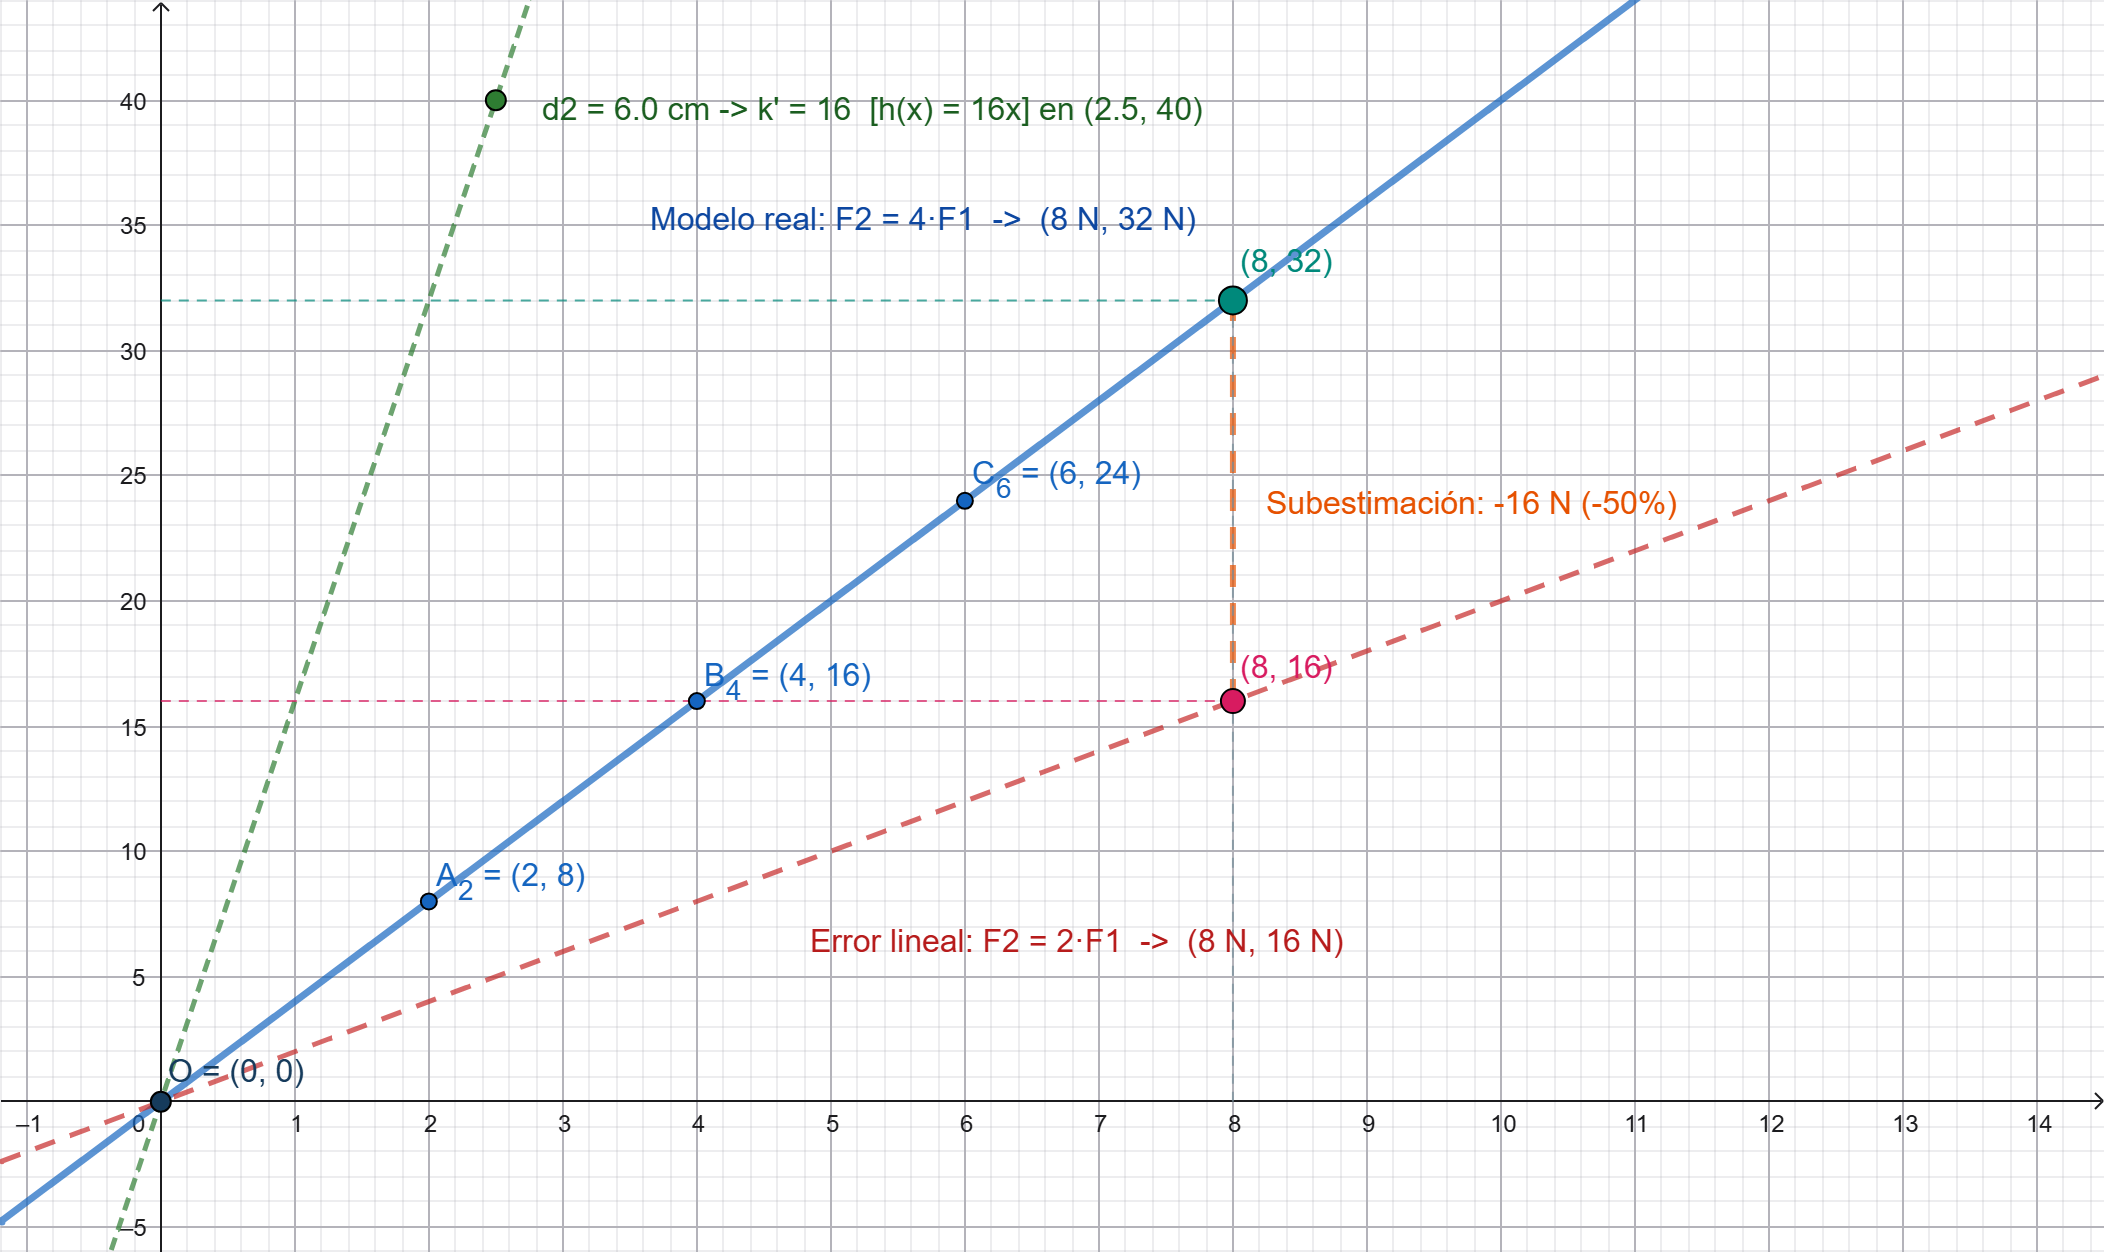
\includegraphics[width=0.98\textwidth,height=5.05cm,keepaspectratio]{img/act6_video_32N.png}
      \end{tcolorbox}
    \end{column}
  \end{columns}
\end{frame}

% =========================================================================
% PAGINA 17 (Beat 16: frame_indicador | indicador_evidencia)
% =========================================================================
\begin{frame}[plain]
  \visHeader{Indicador y Evidencia Observable de Desempeño}{Validación integral: tabla experimental, modelo algebraico y entorno GeoGebra Classic}
  \begin{columns}[T,onlytextwidth]
    \begin{column}{0.56\textwidth}
      \begin{tcolorbox}[viscard=visNavyMid,title={CAPTURA REAL GEOGEBRA CLASSIC $\cdot$ VISTA ALGEBRAICA + GRÁFICA}]
        \centering
        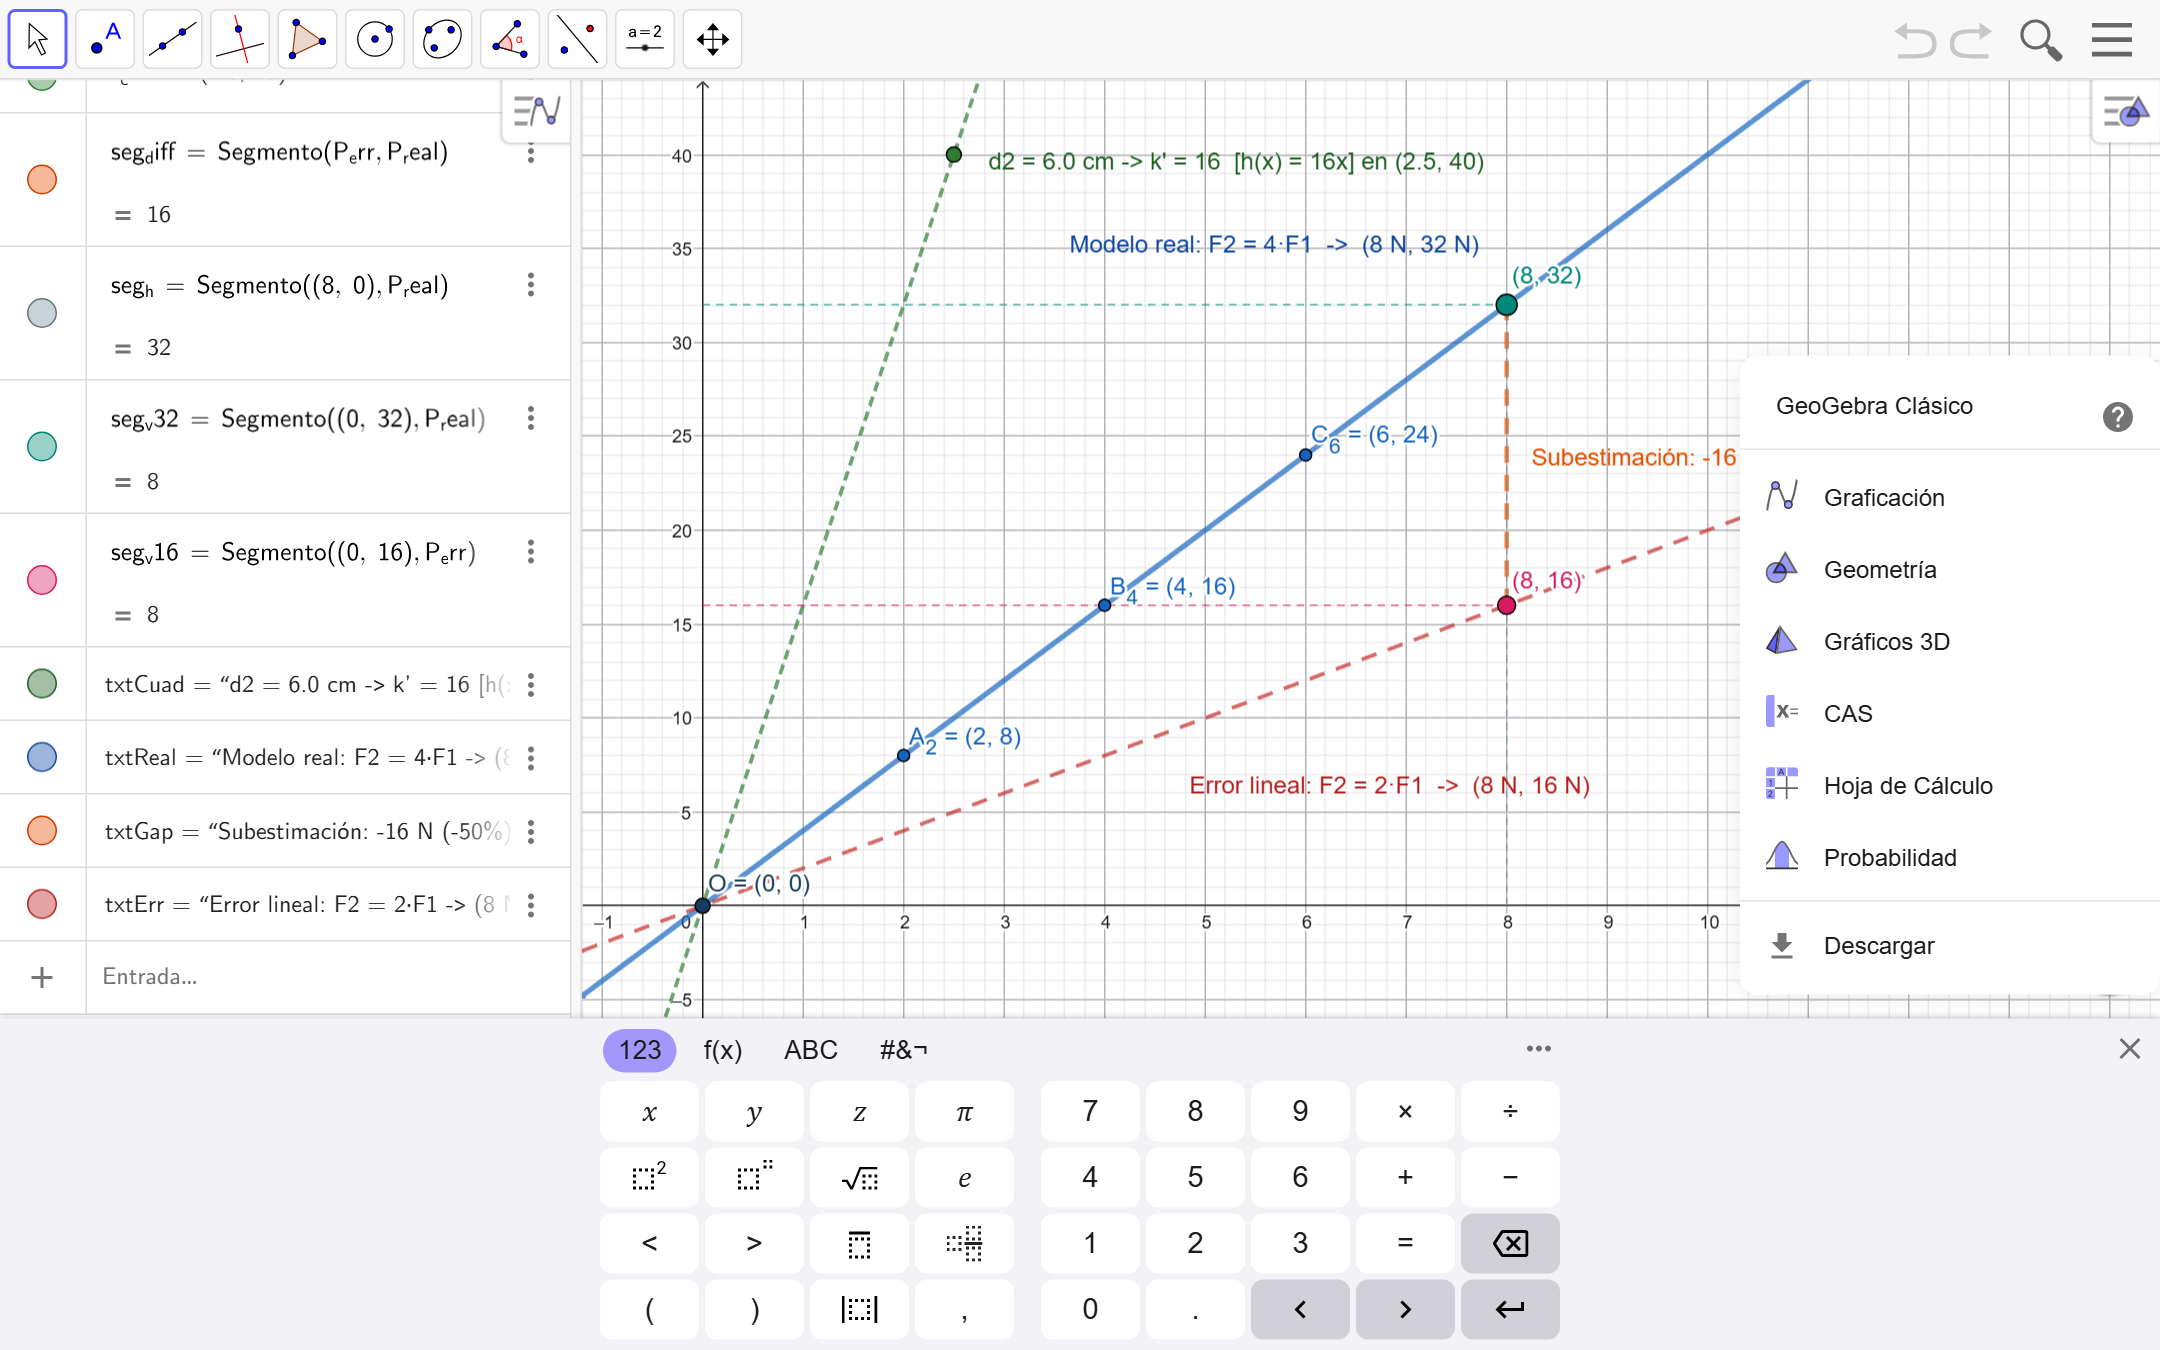
\includegraphics[width=0.99\textwidth,height=5.15cm,keepaspectratio]{img/act6_video_32N_ui.png}
      \end{tcolorbox}
    \end{column}
    \begin{column}{0.42\textwidth}
      \begin{tcolorbox}[viscard=visBlue,title={TABLA DE DATOS VERIFICADA ($k=4$)}]
        \centering\scriptsize
        \begin{tabular}{ccc}
          \toprule
          $F_1$ (N) & $F_2 = 4 F_1$ (N) & Error $2 F_1$ \\
          \midrule
          2 & \textbf{8} & 4 \\
          4 & \textbf{16} & 8 \\
          6 & \textbf{24} & 12 \\
          \rowcolor{visTeal!15} \textbf{8} & \textcolor{visTeal}{\textbf{32}} & \textcolor{visRed}{16} \\
          \bottomrule
        \end{tabular}
      \end{tcolorbox}
      \vspace{0.08cm}
      \begin{tcolorbox}[viscard=visTeal,title={CRITERIOS DE EVIDENCIA LOGRADA}]
        \scriptsize
        \begin{itemize}\setlength\itemsep{2pt}
          \item[\textcolor{visTeal}{$\checkmark$}] Modela en GeoGebra con recta por $(0,0)$.
          \item[\textcolor{visTeal}{$\checkmark$}] Explica físicamente por qué $k = (d_2/d_1)^2$.
          \item[\textcolor{visTeal}{$\checkmark$}] Argumenta la conservación $V_1 = V_2$.
        \end{itemize}
      \end{tcolorbox}
    \end{column}
  \end{columns}
\end{frame}

% =========================================================================
% PAGINA 18 (Beat 17: frame_cierre | sintesis_creditos)
% =========================================================================
\begin{frame}[plain]
  \begin{tikzpicture}[remember picture,overlay]
    \shade[top color=visNavy,bottom color=visNavyMid] (current page.south west) rectangle (current page.north east);
    \draw[white,opacity=0.04,step=0.6cm] (current page.south west) grid (current page.north east);
    \fill[visAmber] (current page.north west) rectangle ([yshift=-0.12cm]current page.north east);
    \node[anchor=north west] at ([xshift=0.52cm,yshift=-0.40cm]current page.north west) {\visualLogo{logo-iiiepe-blanco.png}};
    \node[anchor=north east,fill=visTeal,text=white,font=\scriptsize\bfseries,rounded corners=3pt,inner sep=4pt]
      at ([xshift=-0.52cm,yshift=-0.46cm]current page.north east) {SÍNTESIS FINAL $\cdot$ TRABAJO FINAL SD26};
  \end{tikzpicture}
  \vspace*{1.02cm}
  \begin{center}
    {\color{white}\fontsize{15}{18}\selectfont\bfseries Tres Leyes Clave para Enseñar Proporcionalidad con Sentido Físico}
  \end{center}
  \vspace{0.10cm}
  \begin{columns}[T,onlytextwidth]
    \begin{column}{0.32\textwidth}
      \begin{tcolorbox}[enhanced,colback=visNavyMid,colframe=visCyan,boxrule=1.2pt,arc=4pt,left=6pt,right=6pt,top=6pt,bottom=6pt,height=2.85cm]
        \centering
        {\color{visFluidLight}\scriptsize\bfseries 1. PRINCIPIO DE PASCAL}\\[0.15cm]
        {\color{white}\large $P_1 = P_2 \Rightarrow \dfrac{F_1}{A_1} = \dfrac{F_2}{A_2}$}\\[0.15cm]
        {\color{white!80!visPaper}\tiny El fluido transmite presión íntegra en todas direcciones.}
      \end{tcolorbox}
    \end{column}
    \begin{column}{0.32\textwidth}
      \begin{tcolorbox}[enhanced,colback=visNavyMid,colframe=visAmber,boxrule=1.2pt,arc=4pt,left=6pt,right=6pt,top=6pt,bottom=6pt,height=2.85cm]
        \centering
        {\color{visAmber}\scriptsize\bfseries 2. GANANCIA CUADRÁTICA}\\[0.15cm]
        {\color{white}\large $k = \left(\dfrac{d_2}{d_1}\right)^2$}\\[0.15cm]
        {\color{white!80!visPaper}\tiny Duplicar el diámetro cuadruplica el área y la fuerza ($2^2 = 4$).}
      \end{tcolorbox}
    \end{column}
    \begin{column}{0.32\textwidth}
      \begin{tcolorbox}[enhanced,colback=visNavyMid,colframe=visTeal,boxrule=1.2pt,arc=4pt,left=6pt,right=6pt,top=6pt,bottom=6pt,height=2.85cm]
        \centering
        {\color{visTeal!40!white}\scriptsize\bfseries 3. CONSERVACIÓN}\\[0.15cm]
        {\color{white}\large $F_1 \Delta x_1 = F_2 \Delta x_2$}\\[0.15cm]
        {\color{white!80!visPaper}\tiny Ganar fuerza $k$ veces implica reducir el recorrido $k$ veces.}
      \end{tcolorbox}
    \end{column}
  \end{columns}
  \vspace{0.18cm}
  \begin{tcolorbox}[enhanced,colback=white!10!visNavy,colframe=visSteelDark,boxrule=0.8pt,arc=4pt,left=8pt,right=8pt,top=4pt,bottom=4pt]
    \color{white}\scriptsize
    \textbf{Idea fuerza:} \textit{El aprendizaje matemático cobra sentido cuando cada ecuación explica un fenómeno real del mundo.}\\[2pt]
    \color{visFluidLight}\tiny \textbf{Referencias:} Mendoza, T. \& Block, D. (2010). \textit{La proporcionalidad en secundaria}; Serway, R. (2018). \textit{Física}; SEP (2022). \textit{Plan de Estudio NEM}. \quad|\quad \textbf{Autor:} Mtro. Martín Jonathan de la Cruz Muñoz (00874).
  \end{tcolorbox}
\end{frame}

\end{document}
